\chapter{A Functional Reference Architecture for Aggregators}\label{app:etfa2015}

\textbf{Authors:}\\
	Daniel~Esteban~Morales~Bondy\\
	Kai~Heussen\\
	Oliver~Gehrke\\
	Anders~Thavlov

\noindent
\textbf{Published at:}\\
Emerging Technologies and Factory Automation (ETFA), 2015 IEEE\\
Luxembourg, Luxembourg

\noindent
	\textbf{Abstract:}\\
Aggregators are considered to be a key enabling technology for harvesting power system services from distributed energy resources (DER). As a precondition for more widespread use of aggregators in power systems, methods for comparing and validating aggregator designs must be established. This paper proposes a functional reference architecture for aggregators to address this requirement.


\section{Introduction}
\newchapter{T}{he} increase of electricity production from fluctuating renewable sources is creating a need for new ways of operating the power system. Demand response (DR), i.e. the exploitation of flexibility in electricity consumption, is considered a promising technology for mitigating this problem. However, a significant part of the DR potential exists in distributed, small and medium-sized loads. It is not practical for a power system operator to interact directly with all these flexibility assets. The role of aggregators is the creation and management of a portfolio of flexibility assets and  representation of this combined flexibility to a system operator and/or market.

System operators today rely on generators for ancillary services to maintain reliable system operation. Generators undergo validation tests and continuous monitoring on the generator site. With ancillary services provided by aggregators, similar validation and performance requirements will have to be established. However, validation and monitoring requirements cannot effectively be translated from single site monitoring to distributed aggregator control systems, and today's on-site monitoring cannot be scaled to distributed flexibility assets. 

We propose a functional aggregator reference architecture that facilitates specification and validation of aggregator functional requirements and the generic modeling of contractual and verification performance requirements. Application of the proposed functional architecture to  different aggregator designs suggests it as a meaningful benchmark for technology maturity.

% SUGGESTING TO REMOVE THIS PARAGRAPH FOR THE SHORT PAPER
%The paper presents a short overview of the current state of aggregation in Section~\ref{sec:agginsg}. The motivation for the reference architecture are presented in Section~\ref{sec:requirements} and an analysis of the aggregator functionality is presented in Section~\ref{sec:funcdec}. Section~\ref{sec:refarch} presents the proposed framework based upon the functionality analysis, and Section~\ref{sec:applic} shows how the framework can be applied to a set of academic and commercial aggregators.

%usual blabla about Smart Grids, and which problems aggregators are supposed to address in the Smart Grid context (scalability/divide-and-conquer, threshold to market entry, competition and indirectly robustness because of multiple implementations etc.). 
%\begin{itemize}
%\item Commercial aggregators are being developed by multiple parties and see their first field use. All of these are one-off designs.
%\item Performance evaluation and service validation will become important issues to be solved once aggregators are supposed to leave the protected field test environment and enter a competitive market.
%\item However, the wealth of different designs and solutions makes finding a common benchmark for evaluation and validation difficult.
%\end{itemize}
%This paper proposes a generic reference architecture for the performance evaluation of aggregators which can be used for ... and makes ... easier.

%Also, this work can serve as a checklist for companies that seek to start an aggregator business.
%Aggregation of large quantities of small, medium sized loads or a few large loads is a solution for harnessing resources that are useful for maintaining power quality and reliability in power systems with large penetration of fluctuating renewable energy sources.

%#############################################
\section{Aggregation in Smart Grids}
\label{sec:agginsg}
%This is where the state of the art goes:
%\begin{itemize}
%\item what is aggregation in a smart grid context?
%\item What is being aggregated?
%\item What is the purpose of the aggregation (delivery of which product?) 
%\item Which types of design exist (examples, not categorisation yet - we'll do that later) Examples
%\item Outcome: Why are aggregators an issue in smart grids?
%\end{itemize}
We refer to the concept of aggregation as the  creation and (commercial and technical) management of a portfolio of flexibility assets with the objective of offering the combined flexibility as a commercial service. The business role and technical function of performing aggregation is referred to as the Aggregator. In literature and business context use of these and related terms is not yet harmonized.
\begin{figure}[t!]
\centering
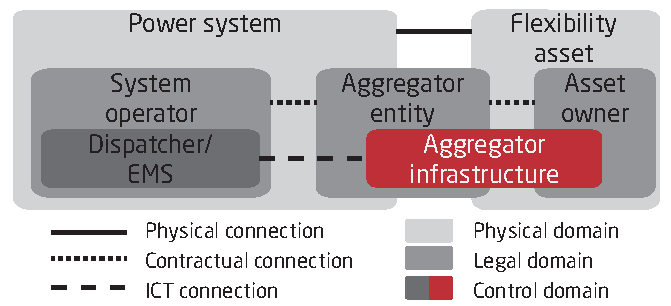
\includegraphics[width=1.0\columnwidth]{etfa2015/domains.eps}
\caption{The aggregator concept across domains.}
\label{fig:domains}
\vspace*{-5mm}
\end{figure}
\subsection{Clarifying the Aggregator concept}\label{subsec:clarifying}
The term \emph{aggregation} has different relevant interpretations in business, information technology,  control, as well as in the physical power system domain. Our concept of aggregators is illustrated in Fig.~\ref{fig:domains}, defining aggregators as a business role, aggregator entity, as well as a technical aggregator infrastructure.

The physical domain addresses the electrical interactions between flexibility assets (also referred to as DER) and power system. Whereas aggregation with respect to physical topology is a common concept (e.g. microgrids, cells), in our understanding, aggregators are not bound to aggregation with respect to physical network topology. 
%The aggregator is only reflected in this level by the manipulation of the interaction between the flexibility assets and the power system.

In the legal and business domain, an aggregator entity is an intermediary, maintaining contractual relations with flexibility asset owners and system operators (as receivers of flexibility services). The aggregator entity assumes legal responsibility for the delivery of a contracted service. The aggregator role may be filled by new independent market actors or be part of existing actors, such as utilities or balance responsible parties.

In the control domain, the aggregator infrastructure coordinates the behavior of flexibility assets. The control domain requirements are formulated as \emph{flexibility services} to system operators and \emph{asset management services} towards asset owners. Tracing these requirements for architectural validation and performance validation in the aggregator infrastructure is the focus of this paper.

The proposed aggregator concept is implementation agnostic and focused on formulation of functional requirements.

\subsection{The aggregator concept in technical literature}
There is no unanimous definition in literature of what could be considered standard functionality of an aggregator. This is reflected by the wide variety of aggregator designs\fcite{kok2005powermatcher,han2010development,sortomme2011optimal,costanzo2013coordination}, which differ in capabilities and purpose, and which use different (often implicit) criteria for classification.

Aggregators are commonly classified by control scheme into autonomous, indirect, transactional and direct control \fcite{Kosek}. Another classification emphasizes the commercial or technical focus of aggregators, referring to \emph{commercial} and \emph{technical} virtual power plants (CVPP and TVPP) \fcite{fenix2009}; however, as both types require business and technical functionality, the CVPP/TVPP distinction expresses a difference in degree and is not categorical. An advanced aggregator realizing the full functionality spectrum as \emph{Dynamic VPP} (DVPP) has been formulated in other work\fcite{niesse2014conjoint}. 
The proposed concept of aggregation encompasses all of the above but focuses on functional requirements for service provision, not business logic.

\subsection{Aggregator Business Harmonization and Standardization}
Whereas aggregator functionality is becoming a shared concept, there are still many models describing a) which stakeholders may benefit from the flexibility service, b) the form of the flexibility service, c) which stakeholders (are allowed to) perform aggregation and who should receive compensation \fcite{eurel-aggr} and d) how to harmonize the interaction between aggregators and aggregated units.

With respect to a), market models are being revised and new service models introduced to assign a value to flexibility (either directly to system operators as ancillary service, or as enhancement of flexibility of existing portfolios). The form of the service, b), is often formulated as an abstract flexibility service, a trade-off between both grid needs and generalized resource characteristics. Regarding d), many aggregators use proprietary communication, loosely based on standards (e.g. IEC61850 or IEC 60870-5-104; increasingly also OPC-UA); harmonization efforts in Europe continue to be addressed in the Smart Grid Coordination Group (SGCG) under EU Mandate M/490. A successful interoperability effort in this domain is the OpenADR standard published also as IEC PAS 62746.10-1. Meanwhile the IEC TR 62357 \emph{Reference Architecture to Smart Grid Information Exchange} is under revision. The reference architecture presented here focuses, within the Smart Grid Architecture Model\fcite{SGAM}, on functional interoperability for aggregators (field to operation zones; DER and customer domains) supporting interactions with System Operators, market actors, and devices at process level.

%\noindent\rule{4cm}{0.4pt}\\
%\textcolor{red}{(the follwoing defintioins belong into this section)}\\
%DEFINITION\\
%LEGAL\\
%Aggregator Role $\surd$\\
%Flexibility Asset Owner Role $\surd$\\
%SOFTWARE DOMAIN\\
%Virtual Nodes  (agents, processes) $\surd$ \\
%aggregator-side $\surd$ \\
%asset-side $\surd$ \\
%PHYSICAL DOMAIN \\
%Aggregator Site\\
%Flexibility Asset $\surd$ \\
%Device Interface $\surd$ \\ 

%#############################################
\section{The Need for an Aggregator Reference Architecture}
\label{sec:requirements}
%The power system is experiencing a paradigm shift. 
Existing concepts and methods for benchmarking and generator validation/certification cannot readily be translated from the (bulk) generator based paradigm to the distributed paradigm of aggregators and flexibility services. Historically, ancillary services have been defined using a physical understanding of generator capabilities. This definition is moving towards technology-agnostic service models.
Service verification has been done through on-site measurements, which is infeasible with thousands of units participating in service provision.  

The definition of a reference architecture for aggregators addresses these three issues, and enables benchmarking of aggregator architectures.
A reference architecture ``captures the essence of existing architectures, and the vision of the future needs and evolution to provide guidance to assist in developing new system architectures.''\fcite{cloutier2010concept}. It should provide: 
\begin{itemize}
\item a common lexicon and taxonomy,
\item modularization and the complementary context, and
\item a common (architectural) vision.
\end{itemize} 

%1) new industry -> benchmark, kpis certification is needed, since they cannot be translated from the old industry 
%
%2) service verification is different -> traditionally expensive measuring equipment. new method is needed for new architecture
%
%3) technology agnostic service models, rather than technology based services. Need an architecture to standardize context
%The common lexicon and taxonomy allows for precise discussion and a common understanding of what an aggregator is and can do. The establishment of these two concepts is started in Section~\ref{subsec:clarifying}, where the context of the aggregator is also discussed.% and further refined throughout the paper. 
Various types of aggregator implementation exist, realizing different design ideas for different sets of requirements. These requirements -- and consequently the designs derived from them -- are unlikely to converge towards a single solution because of the tradeoffs involved, e.g. scalability and complexity. A common lexicon and taxonomy is a minimal precondition for aggregator comparison.
If a reference architecture is to be used to describe many of these different designs, it must be highly modular. In practice, the \emph{general} functionality of an aggregator must be broken down into small enough functions in order for these functions to be usable as building blocks for the reconstruction of the \emph{particular} functionality of a given implementation. 
The functions are arranged in a reference architecture such that metrics can be assigned to individual functions. In this way, the reference architecture can be used for validation of the aggregator. Our architectural vision accounts for the need for verifying distributed flexibility services.

%Implementability (discuss what that means in this context?)

%The methodology for the analysis is the following:
%\begin{itemize}
%	\item We have analyzed different aggregator architectures from the literature, as well as the experience gained through the practical implementation of an aggregator in our laboratory, and extracted the essential functionalities necessary for the working of the aggregator. These functionalities are independent from aggregator/control architecture.
%	\item We analyze the functions and their relationships, as well as the level of complexity we can foresee.
%	\item Synthetize the results into a reference architecture. 
%	\item Validate by mapping different architectures into the framework.
%\end{itemize}


%This is still part state of the art, so this and the previous section together shouldn't be too long)
%\begin{itemize}
%\item \textit{The method}
%\item Why would somebody want to evaluate aggregator performance?
%\item Which methods/approaches for performance evaluation exist or are being discussed?
%\item What is missing? (A reference architecture of course, but why?)
%\end{itemize}

%#############################################
\section{Functional decomposition}
\label{sec:funcdec}
An aggregator is a complex system of interacting functions. In the following definitions, we abstract from implementation details, e.g. centralized vs. distributed systems, and focus purely on the purpose of the functions. 

% EXTERNAL INTERFACES
%\subsection{Service Interface}
\textbf{A. Service Interface}
The service interface translates the contractual agreements between the aggregator and its clients into a service model containing quantifiable and measurable service requirements and a set of performance criteria. This service model is then used to map incoming service requests to control domain signals such as control variables, constraints or control parameters.


% Monitoring & Supervision modules
%\subsection{Performance Monitoring}
\textbf{B. Performance Monitoring}
The performance monitoring function collects data from which the behaviour of individual clients can be derived. The data is analyzed to determine the performance of a client, and its compliance with the contracted flexibility service. This analysis may be internal to the performance monitoring function, or it may simply serve as a data gatherer for an external entity.


%\subsection{Supervision and Resource Handling}
\textbf{C. Supervision and Resource Handling}
The aggregator must maintain an overview of available client resources and their status. By comparing the communication status and monitored performance of individual clients to the control signals sent by the aggregator, the supervision function determines whether clients perform according to their contract. It may temporarily or permanently exclude non-compliant clients from the pool of available resources.


%\subsection{Operator Interface}
\textbf{D. Operator Interface}
Although the power system is moving towards automated solutions, decision-making on critical issues is the responsibility of human operators. The aggregator architecture must support decision-making by presenting operators with the necessary information, and facilitating operator input and intervention.  %\textcolor{red}{(Incomplete/rewrite!)}


% Control-related
%\subsection{Control}
\textbf{E. Control}
The control function is in charge of generating the appropriate control domain signals for the portfolio. Depending on the control architecture, the control logic may be distributed between physical entities. The concept of a control domain signal covers several kinds of signals, including, but not limited to control inputs to DERs, coordination messages for distributed control and reference signals for hierarchical controllers.


%\subsection{Flexibility Monitoring}
\textbf{F. Flexibility Monitoring}
In operation, the aggregator must assess the future flexibility of its portfolio in real time; this includes individual DER flexibility as well as the aggregated flexibility of the portfolio. The flexibility assessment can either be based on direct feedback from the DERs or entirely on estimation models (possibly stochastic) if direct feedback is not available.

% Communication
%\subsection{Aggregator-internal communication}
\textbf{G. Aggregator-internal communication}
Except for very few special cases, aggregation will almost always be implemented as a distributed computing system. In its basic form, such a system would consist of one aggregator and a number of clients. This may be extended by stacking multiple levels of aggregation etc. The internal communication function exchanges information between aggregator and clients.


%\subsection{Client management}
\textbf{H. Client management}
The client management function actively or passively tracks the availability of clients. It may also provide a mechanism for the dynamic addition and removal of clients, such as a discovery service, and maintain a protocol for temporarily disabling otherwise available resources. It contributes to resilience and graceful degradation of the portfolio.



%\subsection{External Information Services}
\textbf{I. External Information Services}
To be able to act optimally with respect to both control of its portfolio and trade of electricity in forward markets, aggregators will likely have to rely on different types of information services. Such services include different types of forecasts and measurements in real time and may be provided by either internal processes or by a 3rd party. 


%\subsection{Asset interface}
\textbf{J. Asset interface}
Most aggregators in a Smart Grid context will be used to harvest flexibility from existing energy resources. In most cases communication between aggregator and resource will use a fieldbus-style interface not designed for wide-area communication. The purpose of the asset interface is to maintain communication with a physical unit under aggregator control and provide abstraction from interface details.


% the odd one
%\subsection{Information Exchange}
\textbf{K. Information Exchange}
Virtually any modular software framework contains a facility for information exchange between its components and storage of the overall system state: static data, dynamic data or both. A knowledge exchange may take many different forms, from a collection of object references towards a central or distributed database. 


%#############################################
\section{The Reference Architecture} 
\label{sec:refarch}
% === This is where we collect the knowledge collected in the previous section into the actual architecture and discuss it and its building blocks. (Introduce complexity levels) ===

We have now established a set of functions to serve as building blocks for a reference architecture, but without concern for the relations between these blocks. Next, these relations will be examined; in other words: how could a practical aggregator infrastructure be composed from these function blocks?

\subsection{Function blocks and knowledge exchange diagram}

% === Explain what the function blocks symbolize - and how the location in the function block diagram does not say anything about whether a block exists on the aggregator side, the client side or both. ===

The functions in section \ref{sec:funcdec} generally belong to one of the following categories:
\begin{itemize}
\item functions dedicated to communication between physically separate parts of the aggregator infrastructure or communication with 3rd party entities, i.e. enablers of the distributed nature of the system.
\item functions which perform decisions with regards to flexibility asset behavior and portfolio composition.
\item functions which interpret information and support the decision making functions. 
\end{itemize}
These categories represent requirements for different architectural paradigms: Communication functions are layered or hierarchical, and, in the case of communication between aggregator and client, require an identically layered counterpart at the opposite end. The decision making and interpreter functions on the other hand require many hierarchical and non-hierarchical consumer-producer relations. % The interpreter functions generally exist in direct relationship with the decision making functions. %The knowledge exchange function, storing the different elements of system state, provides a link between these two worlds.  
Figure~\ref{fig:functiondiagram} shows an overview of the relationships between functions according to the above concept.

\begin{figure}[htb]
\centering
\includegraphics[width=1.0\columnwidth]{"etfa2015/diag_simple"}
\caption{Each function outputs distinct kinds of data which are used by the other functions in different ways according to the aggregator implementation.}
\label{fig:functiondiagram}
\end{figure}

\subsection{Principles of distribution of functions}

While figure \ref{fig:functiondiagram} depicts the relationship between aggregator functions, it does not include information about the physical distribution of these functions between the asset side and the operator side of the aggregator infrastructure. This distribution is highly specific to the individual design and e.g. its degree of centralization (see section \ref{sec:applic}).

In an actual implementation, several of these functions require corresponding instances on each side, effectively forming a communication stack. 

The functions exhibiting these properties are:
\begin{itemize}
\item the internal aggregator communication function which provides the link between the two substacks. In many cases, this function will make use of a full OSI-layered stack in which the internal aggregator communication function provides the application layer,
\item the client management function, implementing management protocols which would typically require a corresponding instance on the client side, and
\item the knowledge exchange function which exchanges information with its client side counterpart independent of client management mechanisms.
\end{itemize}

All other functions, with the exception of the asset interface, may appear either on the operator side, on the asset side, or shared between both sides, depending on the implementation.

%#############################################
\section{Case studies} 
\label{sec:applic}

A number of existing aggregator designs -- commercial as well as academic -- have been mapped to the model in order to test its viability. Two cases with different design philosophies are presented here in order to illustrate the distribution of functionality between the operator and the asset side, and the information flow between the functions:
\begin{itemize}
	\item \emph{Power Hub} is an aggregator developed by Dong Energy in Denmark. It is used to control distributed generation and load in order to sell flexibility services to the ancillary power market (Figure~\ref{fig:powerhub}).
\item \emph{Open Energi} is a British company selling flexible consumption from industrial loads as an ancillary service. The aggregator functions are distributed between an operator node at a control center and asset nodes on custom hardware deployed at customer sites (Figure~\ref{fig:openenergi}).
\end{itemize}

The most significant difference between the two designs is the degree of autonomy of the asset node. The Power Hub concept is based on a centralized design which mainly uses the asset node as a communication gateway and places flexibility monitoring and control at the central operator site. This is also where external information such as market data is available through the information services function.
The Open Energi controller acts on quantities measurable at the asset site and does not require external information; this allows control and flexibility monitoring to be placed at the asset node, leaving only supervisory functions at the operator site.

Both designs can be split into functions according to the subdivision proposed in section \ref{sec:funcdec}.

\begin{figure}[htb]
\centering
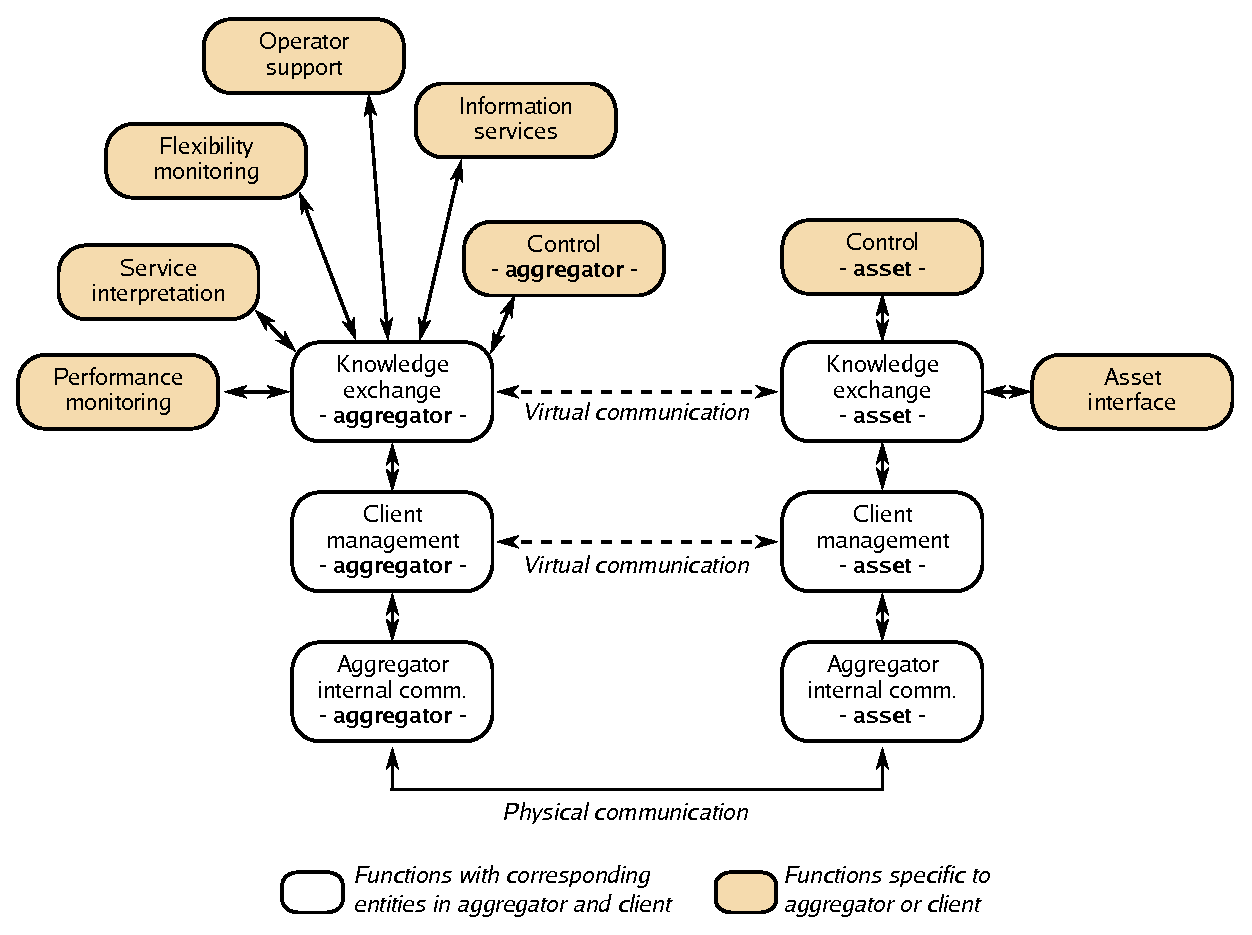
\includegraphics[width=0.65\columnwidth]{etfa2015/stackdrawing_powerhub.eps}
\caption{Distribution of functions for the Power Hub aggregator}
\label{fig:powerhub}
\vspace*{-5mm}
\end{figure}
\begin{figure}[htb]
\centering
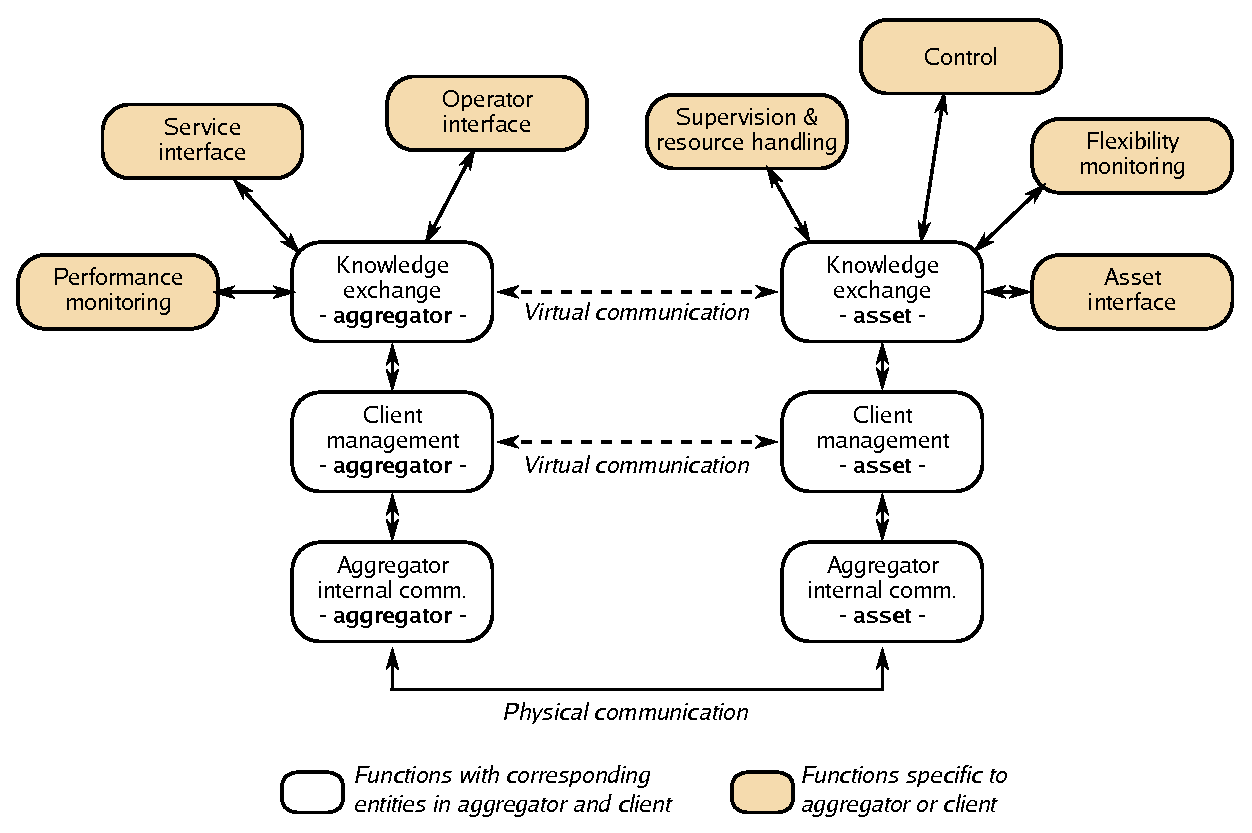
\includegraphics[width=0.65\columnwidth]{etfa2015/stackdrawing_openenergi.eps}
\caption{Distribution of functions for the Open Energi aggregator}
\label{fig:openenergi}
\vspace*{-5mm}
\end{figure}



%#############################################
\section{Conclusion and further work}
\label{sec:etfa2015:conclusion}
A reference architecture for the validation and comparison of aggregators has been presented. While the general framework has been established and successful mapping tests to a number of real-world aggregator designs have been performed, many details are still work in progress.
The next steps towards completion will be the development of performance indicators for the individual functions and the establishment of a process for aggregator comparison and performance validation.

%Review 1: As the goal of the paper is to develop a reference archcture, please elaborate on reference architectures in general and on the SGAM in particular.

%
%Review 2: The WIP-paper presents a high-level reference archcture for the validation and comparison of aggregators for power system services from distributed energy resources. Based on a functional decomposition of practical implementations a reference architecture is developed. It is validated against two practical implementations (power hub and open energi). 
%
%The value of a reference archcture for the crucial role of aggregators such as this is obvious but the developed architecture needs to be validated with more practical examples. How and if this architecture may be used performance evaluation, comparison or even optimization of aggregators remains to be proven. But the paper definitely meets the requirements of a WIP contribution.

%Review 3:	The concept of the reference archcture is nicely introduced and explained. Since it is a work in progress paper a more detailed presentation of future work would be appreciated.

%#############################################
\section*{Acknowledgment}
Parts of this work are supported by the Programme for Energy Technology Development and Demonstration (EUDP) and Innovation Fund Denmark through the iPower project.

